\chapter{相关研究}

目前实际的分布式存储系统经常独立地安排每个修复任务,鲜有考虑到任务彼此的影响。
这些分布式的修复任务共享着底层基础设施的网络、计算和存储资源,这就造成了数据流之间的干扰,导致系统资源利用率低下。
为了缓解这一问题,\citet{popa2013elasticswitch}提出了Elasticswitch,一种可以在各个服务器之间分配带宽的技术。
通过这一技术,将服务器的总带宽资源进行整合,可以为每个修复任务分配必要的网络带宽。此外,系统中主要有三种任务需要优化执行,
其中包括修复任务调度、调度数据的选择以及不同网段的后台修复任务的带宽分配。因此,\citet{li2018joint}提出了LSPT
(Linear Programming for Selected Tasks)在满足数据放置、网络拓扑结构以及带宽限制的条件下,最大限度地增加
满足时间限制的修复任务数。为了最佳地安排每个任务,LSPT共同解决了
(1) 确定用于产生修复流量的纠删码块的选择问题,
(2) 在修复任务之间分配TOR交换机和聚合交换机带宽的带宽分配问题,以及
(3) 根据最后修复时间限制安排任务的调度问题。假设一个数据存储中心的一个聚合交换机连接着$u$个机架交换器(Top-of-Rack)。
$r$个存储节点($\mathcal{R}=\{1,2, \ldots, r\}$)放置在$u$个机架内($\mathcal{U}=\{1,2, \ldots, u\}$)并且每个
TOR交换器。同一个机架内所有的节点的修复流量不需要经过聚合交换机,而不同机架上的存储节点之间的流量则不需要经过两个
TOR交换机和聚合交换机。每份文件$i$用($n_i, k_i$)纠删码进行存储,保证为MDS(Maximum-Distance-Separable)码,确保
$n_i$中的任意$k_i$块可以重建文件$i$。此问题可以描述为,令$\mathcal{A}=\left\{A_{1}, A_{2}, \ldots, A_{m}\right\}$表示
为系统后台任务的集合,诸如备份,修复和数据再分配。对于每个任务$A_i$,相应地有关联参数包括数据块分发源$n_i$(表示为
$o_{i, 1} \in \mathcal{U}, o_{i, 2} \in \mathcal{U}, \ldots, o_{i, n_{i}} \in \mathcal{U}$),分发接收节点(表示为$p_{i} \in \mathcal{U}$),
需要获取的块个数$k_i$,每个块的大小$v_i$,任务开始时间$s_i$,以及任务的终止时间$d_i$。任务的开始时间和结束时间用秒作为单位,
满足$0 \leq s_{i} \leq d_{i}$。不失一般性,考虑带有时间段的系统,假设$y_{i, j}$为编码块的选择变量,例如$y_{i, j}=1$表示
块$j$被选择去执行任务$A_i$,而$y_{i, j}=0$则未被选中。既然块$k_i$必然被选择,则有

\begin{equation}
	\label{eq:2-1}
	\sum_{j} y_{i, j}=k_{i}, \forall i
\end{equation}

为了确定成功完成的任务数,使用二元变量$z_i$来进行表示,当$z_i=1$时任务$A_i$在时间限制内完成,否则未完成。
设$x_{t, i, j}$是在时间段$t$中分配给传输任务$A_i$的$j$块的数据流量的带宽,如果任务在最后期限$d_i$之前完成,
所有的$k$个块传输应该在$d_i$之间完成,即时间限制约束条件为:
\begin{equation}
	\label{eq:2-2}
    \sum_{t=s_{i}}^{d_{i}} x_{t, i, j} y_{i, j} \geq v_{i}, \text { if } z_{i}=1, \forall i, \forall j
\end{equation}

由于每个传输头尾对都有一个预先确定的路线,对于一个给定的任务集,用$RC_g$来表示跨越一个TOR或者聚合交换机$g$的任务或者
块的集合,即$(i,j)\in RC_g$如果任务$i$的块$j$的流量经过了交换机$g$。同样,$SC_h$是经过节点$h$的任务或者块集合。每个
TOR交换机有着容量的限制$CTA$且每个节点有着容量限制$CST$,因此有以下容量限制:

\begin{equation}
	\label{eq:2-3}
    \sum_{(i, j) \in R C_{g}} x_{t, i, j} y_{i, j} \leq C T A, \forall g, t
\end{equation}


\begin{equation}
	\label{eq:2-4}
    \sum_{(i, j) \in S C_{h}} x_{t, i, j} y_{i, j} \leq C S T, \forall h, t
\end{equation}

任务的目标就是要在基于纠删码的存储系统中最大化在时间截止内成功完成的修复任务数。可以看做是一个联合调度和优化问题:

\begin{equation}
    \begin{aligned}
    \label{eq:2-5}
    \max \quad & \sum_{i} z_{i}  \\
    \mbox{s.t.} \quad & \sum_{j} y_{i, j}=k_{i}, \forall i \\
    & \sum_{t=s_{i}}^{d_{i}} x_{t, i, j} y_{i, j} \geq v_{i} z_{i}, \forall i \\
    & \sum_{(i, j) \in R C_{g}} x_{t, i, j} y_{i, j} \leq C T A, \forall g, t \\
    & \sum_{(i, j) \in S C_{h}} x_{t, i, j} y_{i, j} \leq C S T, \forall h, t \\
    \mbox{var.} \quad & x_{t, i, j} \geq 0, y_{i, j} \in\{0,1\}, z_{i} \in\{0,1\}
    \end{aligned}
\end{equation}

其中式~\ref{eq:2-5}的第三行正好对应式~\ref{eq:2-2}任务成功时,即$z_i=1$。


MSR改进。在多个同时发生的故障事件中,单个节点故障的恢复率可达到$98\%$\cite{rashmi2014hitchhiker,xia2015tale}。因此,减少单一故障修复所产生
的延迟对于提高系统性能是至关重要的。\citet{dimakis2007benefits,dimakis2010network}提出了再生码RGC,它可以在存储开销和修复故障节点所需的数据量之间
取得良好的均衡。另一方面,处于最小存储的再生码均衡点的MSR(Minimum Stroage Regenerating)对于大部分纠删码来说是最优的替代选择,因为MSR可以在
最小存储开销下实现最佳修复成本和最大距离可分MDS的特性。MDS属性意味着只要故障块数小于或等于校验块数,那么数据就可以被恢复。然而,MSR码有一些缺点。
(1)大多数现有的MSR码不是系统码,只在编码后存储奇偶校验块信息,因此造成了很高的计算开销;
(2)许多纠删码的存储开销超过系统存储量的2×倍,因此在实际存储系统中没有用处不大;
(3)存储开销低于系统存储量的2×倍的码不仅需要复杂且容易出错的代码策略,而且还需要很高资源的开销。
对于这些问题,Butterfly\cite{pamies2016opening}可以在低存储开销(低于2×倍)的情况下具有实际应用价值的MSR码,
是一种系统化的码,读请求可以直接得到数据而不需要任何解码操作。然而,Butterfly最多只能容忍两个块的故障,因此不能达到高可靠性的标准。
此外,它还存在一个成簇的子包,它将块分成小的片段(最小的编码元素),导致编解码操作中会损失块的位置数据,还会产生数据读取和传输的高通信成本。
\citet{ye2017hybrid}提出了Hybrid-RC利用Butterfly码来对MSR进行优化改进,理论上它是可以在低存储开销和低修复带宽之间取得最优均衡的纠删码。Hybrid-RC使用Butterfly
作为分组校验编码的编码策略,使用伽罗瓦运算进行全局校验码的计算从而保持存储系统的可靠性。与LRC相比,在相同的存储开销下,Hybrid-RC在处理单块故障
恢复时有着更多的数据块参与。每个块的I/O消耗相对减少且数据传输是高度并行的,从而达到了良好的平衡。Hybrid-RC由三个标准化参数组成,$k,l,g$,记为$A(k,l,g)$。
一个条带中有$k$个数据块和$l+g$个校验块,其中$g$个全局校验块通过对所有数据块进行伽罗瓦运算求出。Hybrid-RC将$k$块数据分成$\frac{l}{2}$个组,其中
$l$必须为偶数。当$k$不能被$\frac{l}{2}$整除时且余数为$r$时,那么第0到第$r-1$组应该包含$\left\lceil\frac{2 k}{l}\right\rceil$个块并且每个块被分成了
$2^{\left(\left\lceil\frac{2 k}{l}\right\rceil-1\right)}$个片段。如果不同的组的切片数不同,那么从第$r-1$个到第$\frac{l}{2}-1$个组
应该加倍以保证每个块的存储消耗保持一样。例如,考虑$A(7,4,1)$的Hybrid-RC码,节点中的每个块大小为1GB。第一个组包含4个数据块和2个校验块,所以每个块
有8个切片且每个切片大小为0.125GB。但是,第二个组只有3个数据块,因此每个块有4个切片。为了两个组能保持同样的块大小,第二组的每个块大小需要为0.25GB。
总的来说,不同组的奇偶块构建和块修复是相互独立的。
对于全局编码或修复,最小的操作元素是相同的。因此,不同数量或大小的切片对全局奇偶校验计算是没有影响的。

\begin{figure}[htbp]
	\centering
	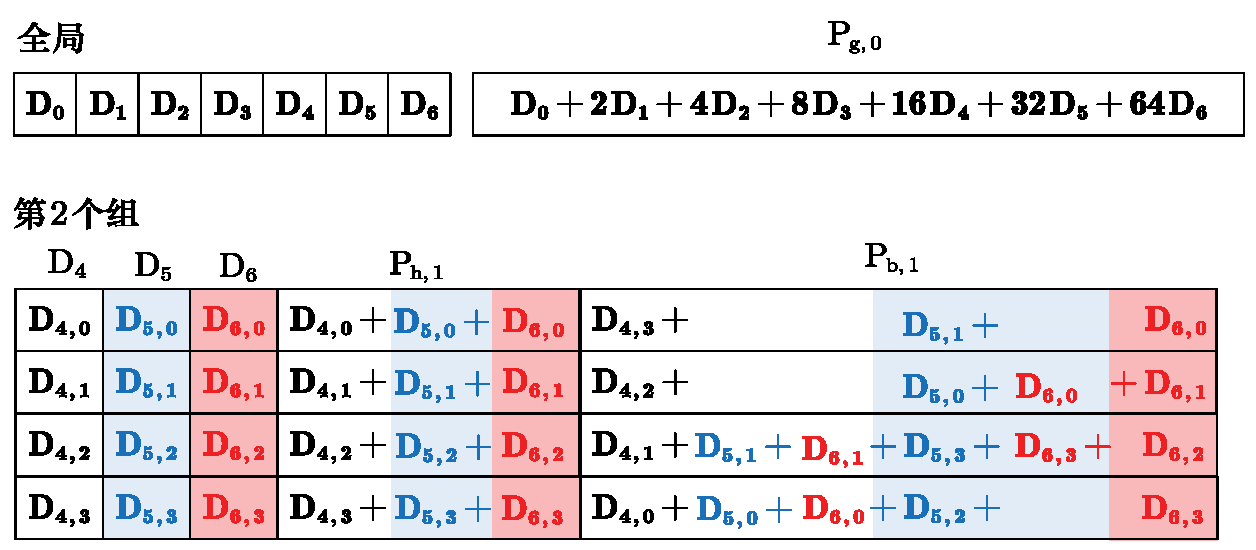
\includegraphics [scale=0.7]{figures/2.1.pdf}
	\caption{(7,4,1)Hybrid-RC}
	\label{fig:con-2.1}
\end{figure}


\section{基于感知修复的研究现状}




\section{基于改进纠删码结构存储数据研究现状}
\section{基于调度优化的数据修复研究现状}
